\newpage\section{Theoretical foundations}

This section represents the theoretical fundamentals of this elaboration by defining the terms \enquote{data analytic}, \enquote{information value chain}, and \enquote{boundaries and conflicts} as they are used in the context of this literature review.

\subsection{Definition of terms}

\subsection{Data Analytics}

The term \enquote{data analytics} originated in the early 2000s and describes an interdisciplinary field that combines areas such as statistics, machine learning, pattern recognition, system theory, operations research and artificial intelligence \parencite{Runkler.2020}. It can be generally defined \enquote{[...] as the application of computer systems to the analysis of large data sets for the support of decisions.} \parencite{Runkler.2020}. This definition showcases the broadness of the topic, as most computer systems process some amount of data and theoretically allow for some kind of decision making. Due to this broad definition, data analytics can cover slightly different subject areas depending on the context it is discussed in. In this elaboration, data analytics refers to the processing of large amounts of data, also referred  to as \enquote{big data}, through mathematical procedures or machine learning methods with the goal of creating new knowledge. In summary, processes that merely prepare or show data are not considered data analytics, but only processes that process data in such a way that new knowledge can be derived from it. This distinction is made to differentiate data analytics from traditional data processing areas like business intelligence. The goal of data analytics, as is discussed in this literature review, is to retrieve some kind of previously unknown knowledge from a set of data. This process can be generally described using the \enquote{information value chain} model. In their research, Abbasi et al. analyze this model in the context of big data in an effort to create an inclusive research agenda for big data in information system research \parencite{Abbasi.2016}.

\subsection{Information Value Chain}

The information value chain (figure \ref{information_value_chain}) is a set of phases that define the transformation of raw data to information and eventually into knowledge. \enquote{Data} describes raw facts without any structuring. Once organized, the processed data represents \enquote{information}. This \enquote{information} is then used to find patterns and draw conclusions. At this time, the information becomes knowledge \parencite{Fayyad.1996}, \cite{Fayyad.1996b}. This knowledge is then used to make \enquote{decisions} and take corresponding \enquote{actions} \parencite{Sharma.2014}. Each phase of the information value chain also includes a different set of technologies and methodologies. For example, the \enquote{data} phase contains technologies and actions regarding the basic storage of data like database systems or data warehouses \parencite{Abbasi.2016}. The conventional version of this information value chain represents an approach that generally explains the processing of data. The main steps of this information value chain are also applicable for big data \parencite{Abbasi.2016}. This general structure of processing data is also supported by literature from the data analytics field \parencite{Runkler.2020}. In addition, the information value chain contains the further phases \enquote{decisions} and \enquote{actions}, which deal with the influence of the processed data. These phases reflect the impact of data analytics, since data analytics is primarily a technology for the decision-making process \parencite{Runkler.2020}. For this reason, the information value chain is a suitable model to structure different phases in the processing of data in the context of data analytics. %For this reason, the literature examined in this paper is structured according to the phases of the information-value chain.



\begin{figure}[]
    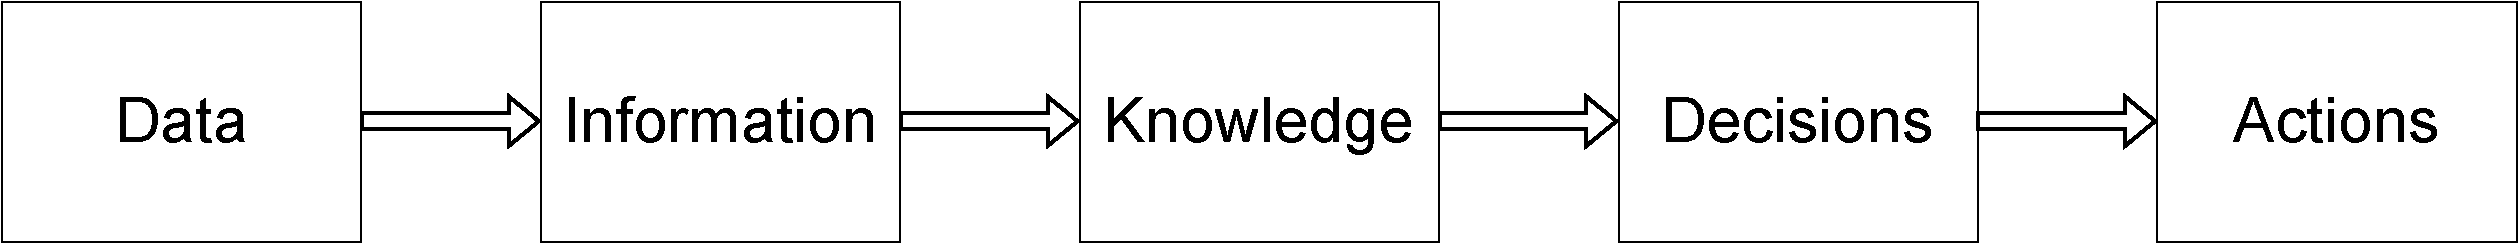
\includegraphics[width=0.99\textwidth, keepaspectratio]{content/02_theretical_foundations/informationValueChain.pdf}
    \caption{Information Value Chain}    
    \label{information_value_chain}
\end{figure}

\subsection{Boundaries and Conflicts in Organizations}

This literature review uses the terms boundary and conflict interchangeably. In order to include as much literature as possible, the criteria for boundaries are kept very general. Prior to conducting the literature review, there was no formal definition of boundaries in the context of data analytics used for the selection of literature. Generally, boundaries are described as \enquote{[...] a real or imagined line that marks the limits or edges of something and separates it from other things or places [...]} \parencite{Hornby.2015}. Based on this general description, the term boundary is defined in the context of this elaboration as any circumstance that leads to a reduction in the effectiveness or efficiency of an organization. %Based on this description, the term \enquote{boundary} is defined in the context of this elaboration as any situation that leads to a reduction in the productivity or effectiveness of a company.
%Simultaneously, the term conflict also describes this circumstance. 
Boundaries and conflicts are therefore used to describe any circumstance that hinders an organization from being perfectly productive. An example of such boundaries or conflicts would be communication issues between different departments, which lead to a reduction of productivity.

\subsection{Design Science Research Methodology}

\subsection{Requirement Engineering}

Die Methodik, um die Anforderungen der Endanwender in dieser Arbeit zu bestimmen, orientiert sich an dem sogenannten \enquote{Requirement Engineering}  \ac{ieee} Standard  für die Analyse und Evaluation von Anforderungsspezifikationen. \parencite[Vgl.][S.2]{SWEBOK.2004} Der Begriff des \enquote{Requirement Engineering}, frei übersetzt mit \enquote{Anforderungsentwicklung}, ist dabei ein englischer Begriff aus der Systemanalyse und wird zur Analyse und Evaluierung von Endanwenderanforderungen genutzt \parencite[Vgl.][S.82-111]{Sommerville.2011} Der \ac{ieee} Standard 610.12-1990 definiert eine Anforderung (englisch \enquote{Requirement}) dabei folgendermaßen: %\newline

\begin{quote}
\textbf{\textit{\enquote{(1) Eine Bedingung oder Fähigkeit, die ein Benutzer benötigt, um ein Problem zu lösen oder ein Ziel zu erreichen. (2) Eine Bedingung oder Fähigkeit, die ein System oder eine Systemkomponente erfüllen oder besitzen muss, um einen Vertrag, eine Norm, eine Spezifikation oder andere formell auferlegte Dokumente zu erfüllen. (3) Eine Dokumentendarstellung einer Bedingung oder Fähigkeit wie in 1 oder 2.}}} \parencite[][S.62]{IEEE.1990}
\end{quote}  %\newline

Die hier verwendete Vorgehensweise orientiert sich allerdings nur in Teilen an diesem Standard, da das \enquote{Requirement Engineering} grundsätzlich ein Teil des Systementwicklungsprozesses ist und sich diese Arbeit nur mit dem Analysieren und Evaluieren von Standardinhaltsanforderungen in einem existierenden System befasst. Deshalb orientiert sich die Definition im Kontext dieser Arbeit an Punkt (1) des \ac{ieee} Standard 610.12-1990 mit dem Ziel, dem Benutzer eine verbesserte Usability zu gewährleisten. Dabei kann das \enquote{Requirement Engineering} in die vier Teilbereiche der Anforderungserhebung, Anforderungsanalyse, Anforderungsspezifikation und Anforderungsbewertung aufgeteilt werden. Bei der Anforderungserhebung werden zunächst die Anforderungen an ein neues Softwaresystem definiert, diese dann analysiert und ausgearbeitet, um sie dann zu dokumentieren und zu evaluieren. \parencite[Vgl.][S.82-111]{Sommerville.2011} Die Anforderungserhebung der Endanwender an das System wird in dieser Arbeit mithilfe einer Umfrage durchgeführt.  Diese Umfrage wird anonymisiert mit Teilnehmern des SAP Enable Now Round Tables stattfinden. In der Anforderungsanalyse wird die momentane Situation der SAP Marketing Cloud betrachtet und mithilfe der Umfrageergebnisse verglichen, um die Anforderungen der Endanwender abzuleiten. Diese Anforderungen werden dann in einem Proof-of-Concept beispielhaft umgesetzt und dazu verwendet, die Anforderungsbewertung durchzuführen. In der Anforderungsbewertung wird dabei der \ac{iso} 9241 Standard\parencite[][]{ISOOrg.2019}  genutzt, um die Verbesserung der Usability zu verdeutlichen. Das Ziel der Umfrage und dieser Arbeit ist es also herauszufinden, wie der SAP Enable Now Webassistent von den Endanwendern genutzt wird und wie der dafür bereitgestellte Standardinhalt in der SAP Marketing Cloud verbessert werden kann.